% !TEX root = Theo_III.tex
\chapter{Magnetostatik}


In den vorigen Kapiteln haben wir uns mit der Elektrostatik beschäftigt und gesehen, wie Ladungen dem Coulombgesetz gehorchen und ein elektrisches Feld hervorrufen, das die Grundgleichungen $\rot \vec {E}=0$ und $\divg \vec {D}=0$ erfüllt.

In der Magnetostatik betrachten wir jetzt stationäre (also nicht zeitabhängige) Ströme und die Kraftwirkung, die sie hervorrufen. Es wird ein Magnetfeld und die Stromdichte eingeführt, was schließlich auf eine integrale und differentielle Formulierung der Grundgesetze der Magnetostatik führt.

Es gibt Ähnlichkeiten zwischen der Elektro- und Magnetostatik, wie zum Beispiel das Abstandsverhalten und die Symmetrie einiger Formeln, aber auch wesentliche Unterschiede, unter Anderem in den Kraftrichtungen und Potentialen.

\section{Strom, Stromdichte und Kontinuitätsgleichung}

Der elektrische Strom $I$ ist als zeitliche Änderung der Ladung definiert,
\begin{equation*}
	I=\frac{\diff q}{\diff t}.
\end{equation*}
Die Einheit ist der Ampère. Aus der Ladungserhaltung folgt, dass der Strom konstant entlang eines Drahts ist.

Außerdem wird die Stromdichte als Strom pro Querschnittsfläche $A$
\begin{equation*}
	\vec {j}=\frac{\text{Strom}}{\text{Fläche}}=\frac{I}{A}\frac{\diff \vec {\vec {r}}}{\diff s}\:\xrightarrow{\Delta  f\diff s=\diff ^{3}r}\: \vec {j}\diff ^{3}\vec {r}=I\diff \vec {r}
\end{equation*}
definiert. Dabei ist $\diff\vec r$ als Leiterelement und $I\diff\vec r$ als gerichtetes Stromelement zu verstehen. Es gilt also 
\begin{equation*}
    I=\int_A \vec j \cdot \diff \vec A,
\end{equation*}
bzw. für eine gleichmäßig auf $A$ verteilte Stromdichte
\begin{equation*}
    I=\vec j\cdot \vec A.
\end{equation*}

Die Stromdichte lässt sich auch ausdrücken durch das Produkt aus Ladungsdichte und Geschwindigkeit,
\begin{equation*}
	\vec {j}=\rho \vec {v},
\end{equation*}
was eine mikroskopische Definition analog zu der der Ladungsdichte erlaubt\footnote{Zur Erinnerung: $\rho =\sum _{i}q_{i}\delta \left(\vec {r}-\vec {r}_{i}\right)$.}:
\begin{equation*}
	\vec {j}=\sum _{i}q_{i}\vec {v}_{i}\delta \left(\vec {r}-\vec {r}_{i}\right)
\end{equation*}
Die Stromdichte zeigt damit in dieselbe Richtung wie der Geschwindigkeitsvektor einer positiven Ladung. 

Zur Herleitung der Kontinuitätsgleichung betrachten wir die zeitliche Änderung der Ladung in einem Volumen $V$:
\begin{equation*}
	\frac{\diff Q}{\diff t}=\frac{\diff }{\diff t}\int _{V}\diff^{3}\vec {r}\rho \left(\vec {r},t\right)=\int _{V}\diff ^{3}\vec {r}\frac{\partial }{\partial t}\rho \left(\vec {r},t\right)
\end{equation*}
Wegen der Ladungserhaltung entspricht dies gerade dem Fluss der Stromdichte aus der Volumenoberfläche $\partial V$ heraus:
\begin{equation*}
	\int _{V}\diff ^{3}\vec {r}\frac{\partial }{\partial t}\rho \left(\vec {r},t\right)=-\int _{\partial V}\vec {j}\cdot \diff \vec {f}=-\int _{V}\diff ^{3}\vec {r}\divg \vec {j},
\end{equation*}
woraus sich die Kontinuitätsgleichung ergibt:
\begin{equation*}
	\frac{\partial }{\partial t}\rho +\divg \vec {j}=0
\end{equation*}
In der Magnetostatik ist $\partial _{t}\rho =0$ und damit
\begin{equation*}
	\divg \vec {j}=0.
\end{equation*}
\section{Leiter und Magnetfeld}

Auf Erde kommen im Wesentlichen zwei natürliche bekannte Magnetfelder vor: dasjenige der Erde und das Magnetfeld von speziellen Mineralen, wie zum Beispiel Magnetit. Hans Christian \O{}rsted entdeckte im 19. Jahrhundert, dass auch stromdurchflossene Leiter ein Magnetfeld erzeugen und André-Marie Ampère entdeckte fast zeitgleich, dass ein Magnetfeld eine Kraftwirkung auf Leiter hervorruft.

Auf ein stromdurchflossenes Volumenelement $\diff V=\diff^3 \vec r$ in einem Magnetfeld $\vec B$ wirkt nach dem folgenden Gesetz eine Kraft\footnote{vergleichlich mit $\vec {F}=q\vec {E}$, also Produkt aus Quelle und Feld in der Elektrostatik. }:
\begin{equation*}
	\diff \vec {F}=(\vec j\times\vec B)\diff V
\end{equation*}
Die Gesamtkraft auf einen ausgedehnten Leiter $V$ ergibt sich durch Integration:
\begin{equation*}
	\vec {F}=\int _{V}\vec {j}\times \vec {B}\diff V
\end{equation*}
Im Spezialfall für einen dünnen Leiter $C$ und ein Leiterelement $\diff\vec r$ ($\diff V = \diff A\diff\vec r$) gilt
\begin{align}
    \label{eq:def_magn_flussdichte}
    \diff \vec F &=I\diff\vec r\times\vec B \\
	\vec {F}&=\int _{V}\vec {j}\times \vec {B}\,\diff A \,\diff\vec r = \int_{A}j\diff A \cdot \int_C \diff\vec r\times \vec B \nonumber\\& = I\int_C \diff\vec r\times \vec B .\nonumber
\end{align}

\begin{figure}[htb]
	\centering
	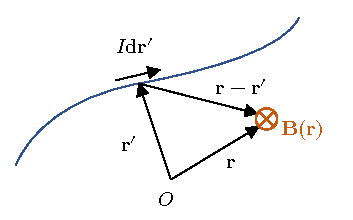
\includegraphics{magnetic_field_conductor_diff_view.pdf}
	\caption{Stromelement $I\diff\vec r$ und Magnetfeld $\vec B$ eines Leiterelements $\diff \vec r$. }
	\label{fig:magnetic_field_conductor_diff_view}
\end{figure}
Wir untersuchen zunächst die magnetische Flussdichte einiger speziellen geometrischen Anordnungen. Es gilt für ein Leiterelement $\diff \vec {r}'$ (dargestellt in \Abbref{fig:magnetic_field_conductor_diff_view}):
\begin{equation*}
	\diff \vec {B}=\frac{\mu _{0}}{4\pi }I\diff \vec {r}'\times \frac{\vec {r}-\vec {r}'}{\left| \vec {r}-\vec {r}'\right| ^{3}}
\end{equation*}
Dieser Zusammenhang ist als Biot-Savartsches Gesetz für Leiter bekannt und ergibt sich aus den Betrachtungen $\left| \diff \vec {B}\right| \propto I\left| \diff \vec {r}'\right| , \left| \vec {r}-\vec {r}'\right| ^{-2}$ und $\diff \vec {B}\perp \diff \vec {r}',\vec {r}-\vec {r}'$. Hier wird außerdem die magnetische Feldkonstante $\mu _{0}\approx 4\pi \cdot 10^{-7}\,\si{\newton\per\square\ampere}$ eingeführt\footnote{Über die Kraft zwischen zwei stromdurchflossene parallele Leiter wurde früher die Einheit Ampère definiert und dabei festgelegt, dass $\frac{\mu _{0}}{4\pi }=\SI{1e-7}{\newton\per\square\ampere}$, aber die magnetische Feldkonstante wurde 2019 umdefiniert auf Basis der Elementarladung und Sekunde, wobei aber die Abweichung extrem gering ist. Damit ist die magnetische Feldkonstante eine experimentell zu ermittelnde Größe geworden. }. Die Flussdichte ist zwar proportional zu $r^{-2}$ wie beim elektrischen Feld einer Punktladung, aber im Gegensatz können isolierte Stromelemente $I\diff \vec {r}$ nicht existieren.

Für das Feld eines unendlich langen, geraden Leiters gilt
\begin{equation*}
    \label{eq:biot_savart}
	B\left(\rho \right)=\frac{\mu _{0}}{4\pi }I\rho \int _{-\infty }^{\infty }\frac{\diff z}{\left(\rho ^{2}+z^{2}\right)^{\frac{3}{2}}}=\frac{\mu _{0}}{4\pi }\frac{I}{\rho },
\end{equation*}


\begin{figure}[htb]
	\centering
	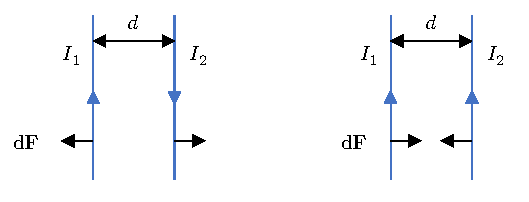
\includegraphics{force_parallel_conductors.pdf}
	\caption{Die Kraft auf parallele, stromdurchflossene Leiter ist anziehend, wenn der Stromfluss in verschiedene Richtungen geht und abstoßend, wenn der Strom in beiden Leiter in der gleichen Richtung fließt. }
	\label{fig:force_parallel_conductors}
\end{figure}

Diese Gleichung beschreibt das historische Biot-Savartsche Gesetz.

Verwendet man Gleichungen \eqref{eq:def_magn_flussdichte} und \eqref{eq:biot_savart}, so erhält man die Kraft zwischen zwei parallelen Leitern mit Abstand $d$ (siehe \Abbref{fig:force_parallel_conductors})
\begin{equation*}
    \frac{\diff\vec F}{\diff z} = \frac{\mu_0}{2\pi} \frac{I_1I_2}d,
\end{equation*}
die orthogonal zum Leiter ist.

Bis zum 20.5.2019 war der Ampère definiert als der Strom, der durch zwei parallele Leiter der Länge $\SI{1}{\m}$ mit $\SI{1}{\m}$ Abstand in gleicher Richtung fließt und eine Anziehungskraft von $\SI{1e-7}{\newton}$ bewirkt. 

Heute gilt
\begin{equation*}
	\SI{1}{\ampere}\equiv \frac{\SI{1}{\coulomb}}{\SI{1}{\s}}.
\end{equation*}
Zwischen beliebigen Leiterschleifen $C_{1},C_{2}$ wirkt eine Kraft von
\begin{equation*}
	\vec {F}_{21}=-\vec {F}_{12}=-\frac{\mu _{0}}{4\pi }I_{1}I_{2}\oint _{C_{1}}\oint _{C_{2}}\frac{\vec {r}_{1}-\vec {r}_{2}}{\left| \vec {r}_{1}-\vec {r}_{2}\right| ^{3}}\diff \vec {r}_{1}\cdot \diff \vec {r}_{2}.
\end{equation*}



\section{Grundgleichungen der Magnetostatik}

Um die Grundgleichungen der Magnetostatik herzuleiten, gehen wir zuerst von dem Stromelement $I\diff \vec {r}$ über in die Stromdichte $\vec {j}\left(\vec {r}\right)$ mit $I\diff \vec {r}=\vec {j}\left(\vec {r}\right)\diff^3 \vec {r}$.

Die Kraft auf ein Stromgebiet ist
\begin{equation*}
	\vec {F}\left(\vec {r}\right)=\int f\left(\vec {r}\right)\diff ^{3}\vec {r}=\int \vec {j}\left(\vec {r}\right)\times \vec {B}\left(\vec {r}\right)\diff ^{3}\vec {r}.
\end{equation*}
Für eine Punktladung $q$, die sich mit Geschwindigkeit $\vec {v}$ bewegt ($\vec {j}=q\vec {v}\delta \left(\vec {r}-\vec {r}\left(t\right)\right)$) gilt speziell
\begin{equation*}
	\vec F\left(\vec {r}\right)=q\vec {v}\times \vec {B}\left(\vec {r},t\right)
\end{equation*}
bzw. allgemein mit einem zusätzlichen elektrischen Feld
\begin{equation*}
	\vec F\left(\vec {r}\right)=q\left(\vec {v}\times \vec {B}\left(\vec {r},t\right)+\vec {E}\left(\vec {r},t\right)\right).
\end{equation*}
Diese Gesamtkraft ist die sogenannte Lorentzkraft.

Integration des Biot-Savartschen Gesetzes für Leiter führt auf\footnote{vergleichlich mit $\vec {E}(\vec r)=\frac{1}{4\pi \varepsilon _{0}}\int \rho \left(\vec {r}\right)\frac{\vec {r}-\vec {r}'}{\left| \vec {r}-\vec {r}'\right| ^{3}}\diff ^{3}\vec {r}'$.}
\begin{equation*}
	\vec {B}\left(\vec {r}\right)=\frac{\mu _{0}}{4\pi }\int \vec {j}\left(\vec {r'}\right)\times \frac{\vec {r}-\vec {r}'}{\left| \vec {r}-\vec {r}'\right| ^{3}}\diff ^{3}\vec {r}'.
\end{equation*}
Wie für das elektrische Feld können wir ein Potential einführen \textendash{} allerdings ist $\vec {B}$ kein Potentialfeld und daher ist das magnetische Potential ein Vektorpotential:
\begin{equation*}
	\vec {B}\left(\vec {r}\right)=\nabla \times \vec {A}\left(\vec {r}\right), \quad\vec {A}\left(\vec {r}\right)=\frac{\mu _{0}}{4\pi }\int \frac{\vec {j}\left(\vec {r}\right)}{\left| \vec {r}-\vec {r}'\right| }\diff ^{3}\vec {r}'
\end{equation*}
Die Divergenz von $\vec {B}$ verschwindet.
\begin{formal}
		Das Magnetfeld hat keine Quellen, $\divg \vec {B}=0$.
\end{formal}
In der integralen Formulierung,
\begin{equation*}
	\int _{V}\divg \vec {B}\,\diff ^{3}\vec {r}=\int _{V}\vec {B}\cdot \diff \vec {f}=0,
\end{equation*}
bedeutet das, dass die magnetischen Feldlinien geschlossen sind. Es gibt folglich keine magnetischen Ladungen, wo die Feldlinien beginnen oder enden.

Für die Rotation der elektrischen Flussdichte gilt
\begin{align*}
	\rot \vec {B}&=\nabla \times \left(\nabla \times \vec {A}\right)=\nabla \left(\nabla \cdot \vec {A}\right)-\nabla ^{2}\vec {A}\\&=\frac{\mu _{0}}{4\pi }\nabla \int \vec {j}\left(\vec {r}\right)\cdot \nabla \frac{1}{\left| \vec {r}-\vec {r}'\right| }\diff ^{3}\vec {r}-\frac{\mu _{0}}{4\pi }\int \vec {j}\left(\vec {r}\right)\nabla ^{2}\frac{1}{\left| \vec {r}-\vec {r}'\right| }\diff ^{3}\vec {r}\\&=0+\mu _{0}\int \vec {j}\left(\vec {r}\right)\delta \left(\vec {r}-\vec {r}'\right)\diff ^{3}\vec {r}\\&=\mu _{0}\vec {j}\left(\vec {r}\right).
\end{align*}

\begin{formal}
	Elektrische Ströme rufen Wirbel in der magnetischen Flussdichte hervor, $\rot \vec {B}=\mu _{0}\vec {j}\left(\vec {r}\right)$.
\end{formal}
Alternativ kann man sagen, dass die Zirkulation entlang der Oberfläche eines Volumens einem Strom durch das Volumen entspricht,
\begin{equation*}
	\int _{\partial F}\vec {B}\cdot \diff \vec {r}=\mu _{0}I.
\end{equation*}
